\chapter{Report Body}
%The central part of the report usually consists of three or four chapters detailing the technical work undertaken during the project. {\bf{\textcolor{red}{The structure of these chapters is highly project dependent}}}. They can reflect the chronological development of the project, e.g. design, implementation, experimentation, optimisation, evaluation, etc (although this is not always the best approach). However you choose to structure this part of the report, you should make it clear how you arrived at your chosen approach in preference to other alternatives. In terms of the software that you produce, you should describe and justify the design of your programs at some high level, e.g. using OMT, Z, VDL, etc., and you should document any interesting problems with, or features of, your implementation. Integration and testing are also important to discuss in some cases. You may include fragments of your source code in the main body of the report to illustrate points; the full source code is included in an appendix to your written report.

In this chapter, I will explain how each of my chosen algorithms work, and how I went around implementing them as a surface-level explanation. I will then briefly compare what challenges I faced for each of my implementations, and how they compare, both performance-wise and with regards to the kinds of layouts they produce, again as surface-level explanations. I go into greater detail on my implementations in the Implementation section, how the level layouts generated in each algorithm compare with each other in the Design \& Specification section, and how each implementation compares overall (and also performance wise) in the Evaluation section. For this project, I chose to use the following 4 algorithms.

\begin{enumerate}
    \item Lindenmayer Systems (or L-Systems)
    \item Perlin/Simplex Noise
    \item Poisson Disk Sampling
    \item Voronoi Cells
\end{enumerate}

\section{Algorithms}

In this section, I will explain how each of the algorithms I implemented work, then I will go into small detail as to how I implemented them. I go into further detail in the ``Implementation" section of this report.

\subsection{Lindenmayer Systems}

Hungarian academic Aristid Lindenmayer devised a mathematical model for the reproduction of fungi in 1967.\cite{LINDENMAYER1968300} His model involved a string of symbols, each unique symbol denoting a specific action and/or branch. Essentially, running that initial string, called the \emph{axiom}, through a set of rules (called a \emph{grammar}) gives us an ever-expanding string that is then taken as instructions to draw something from. Lindenmayer Systems, or L-Systems, have since been used in several scenarios beyond its initial purpose of modelling fungi, from trees to fractals. In video games, they are frequently used to aid in the creation of foliage in several environments, as well as buildings and, here, level layouts.

\subsubsection{A Basic 0L-System}

The most basic form of L-System is a \emph{0L}-System, 0 in this case referring to the fact that the grammar is \emph{context-free}.

For this example\cite{lsyspaulbourke}, consider an alphabet $V$, which consists of the following symbols:

\newcommand{\F}{\mbox{F}}

$$ \F, +, - $$

where $\F$ means ``to go forward", and $+$ and $-$ denote turning right or left (respectively) a set number of degrees $\o$.

Take an axiom $\omega$, for example:

$$ \F+\F+\F+\F $$

And a set of rules $P$ which, in this case, is of size 1:

$$ \F \rightarrow \F+\F-\F-\F\F+\F+\F-\F $$

We can represent this \emph{parametric} L-system in the following form:\cite{enwiki:1124510226}

$$ G = (V, \omega, P) $$

To implement $G$ in Godot, we can take each rule and replace each string in accordance to our one rule, using the replace method, like so:

\begin{figure}[H]
    \centering
    \begin{lstlisting}
string = string.replace(rule["from"], rule["to"]) #Here the rules were stored in dictionaries.
    \end{lstlisting}
    \caption{A line of code that demonstrates directly replacing characters in a string according to our L-System grammar's rules.}
    \label{fig:lsys-snippet-1}
\end{figure}

The first 3 iterations of this operation are shown here:

\begin{figure}[H]
	\centering
	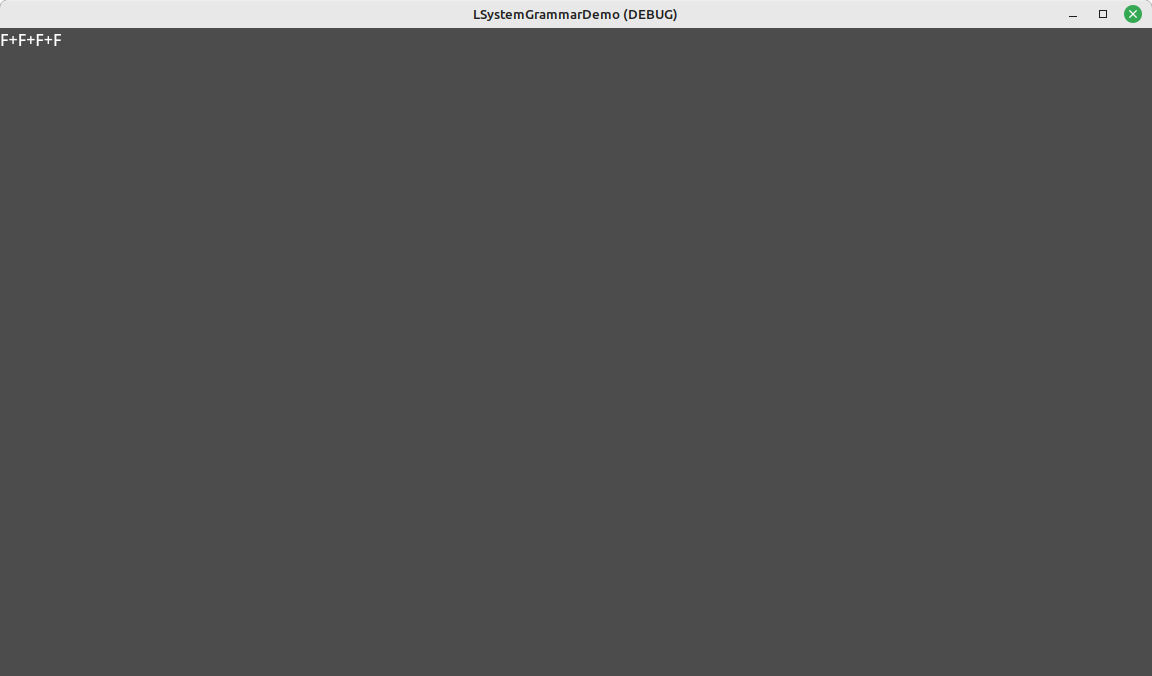
\includegraphics[width=0.5\textwidth]{Images/initial-l-system-iteration-0.png}
	\caption{The axiom of the aforementioned simple L-System with just one rule. String size: 8.\\Source: Own work.}
	\label{fig:lsysiter0}
\end{figure}

\begin{figure}[H]
	\centering
	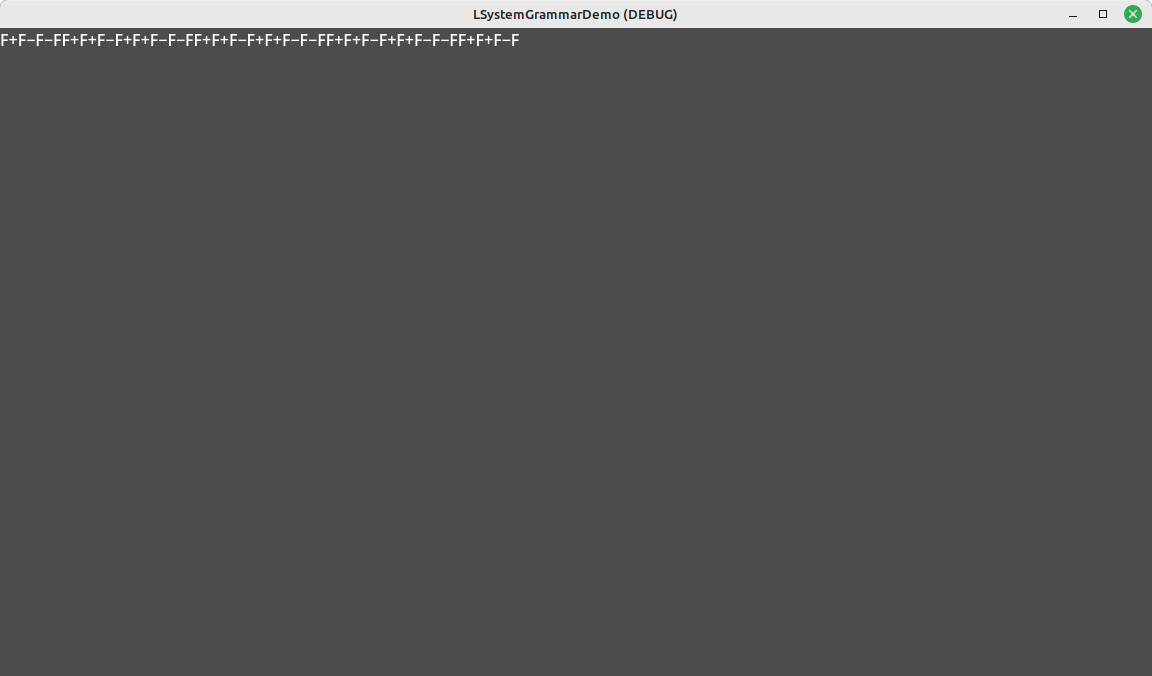
\includegraphics[width=0.5\textwidth]{Images/initial-l-system-iteration-1.png}
	\caption{The first iteration of the aforementioned simple L-System with just one rule. String size: 59.\\Source: Own work.}
	\label{fig:lsysiter1}
\end{figure}

\begin{figure}[H]
	\centering
	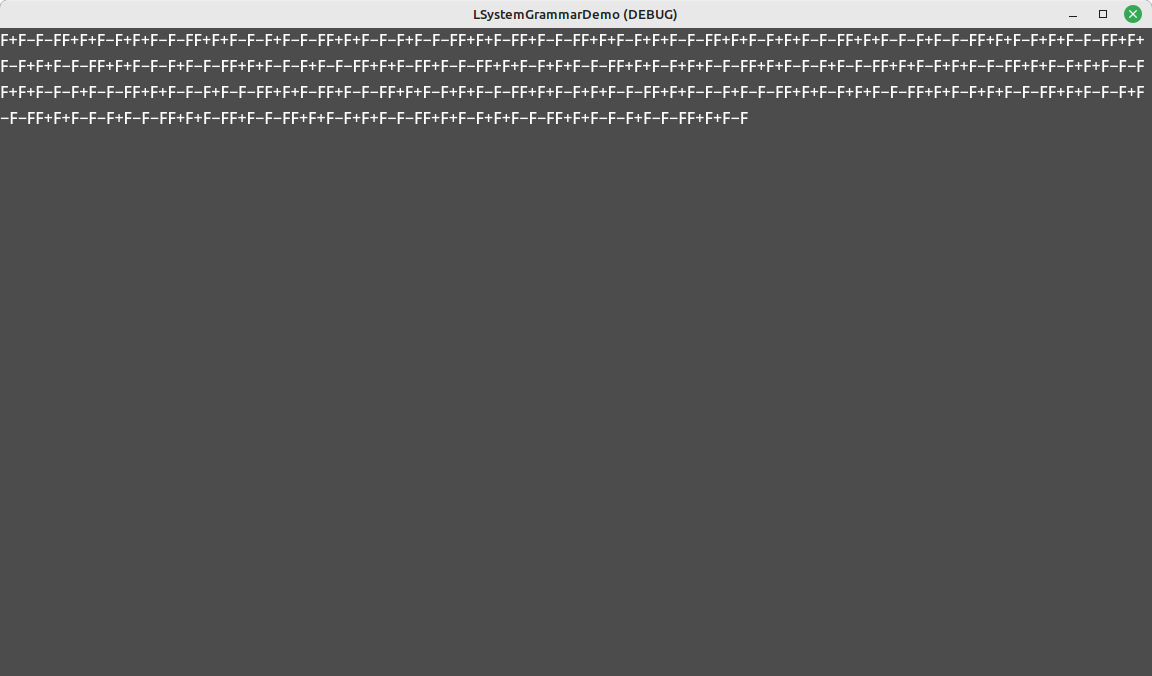
\includegraphics[width=0.5\textwidth]{Images/initial-l-system-iteration-2.png}
	\caption{The second iteration of the aforementioned simple L-System with just one rule. String size: 475.\\Source: Own work.}
	\label{fig:lsysiter2}
\end{figure}

\begin{figure}[H]
	\centering
	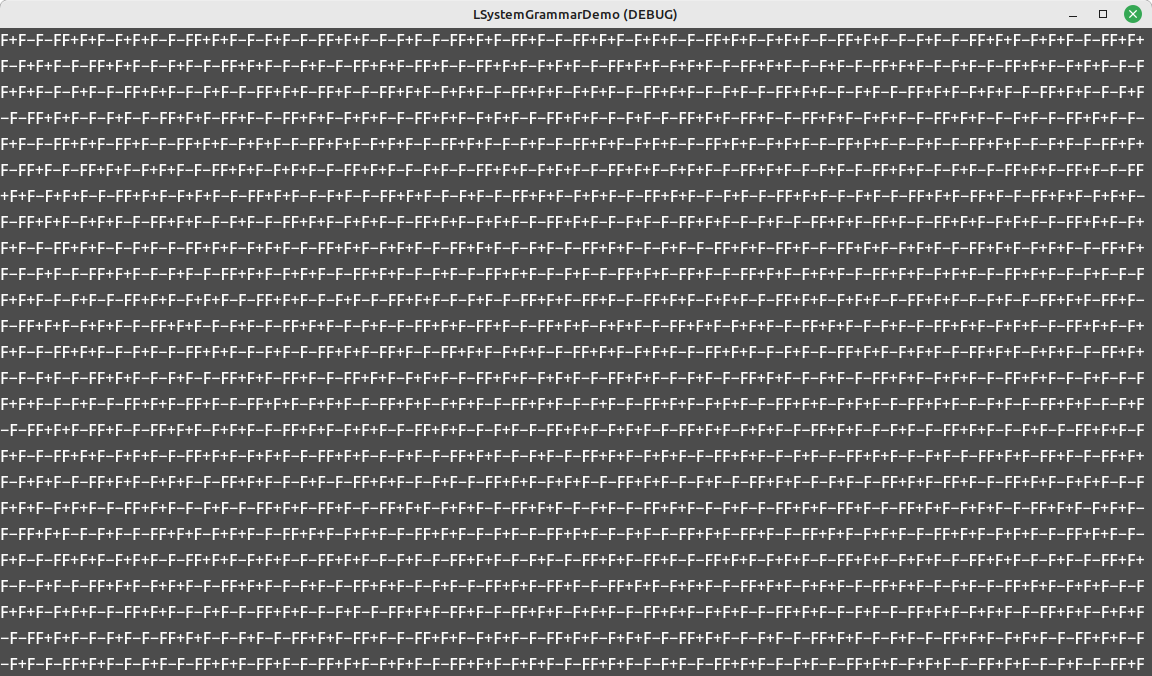
\includegraphics[width=0.5\textwidth]{Images/initial-l-system-iteration-3.png}
	\caption{The third iteration of the aforementioned simple L-System with just one rule. String size: 3803. The string is too large to show in the window, as you can see here.\\Source: Own work.}
	\label{fig:lsysiter3}
\end{figure}

The resulting string can be used to draw a lattice.\cite{lsyspaulbourke} Examples of the above grammar in action are below.

\begin{figure}[H]
    \centering
    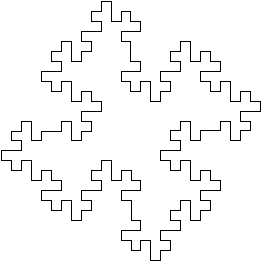
\includegraphics[height=0.25\textheight]{Images/lsys03.png}
    \caption{A lattice generated with the example grammar on a custom-written Classic Mac OS application specifically written for working with L-Systems.\cite{lsyspaulbourke}}
    \label{fig:lattice1}
\end{figure}

\begin{figure}[H]
    \centering
    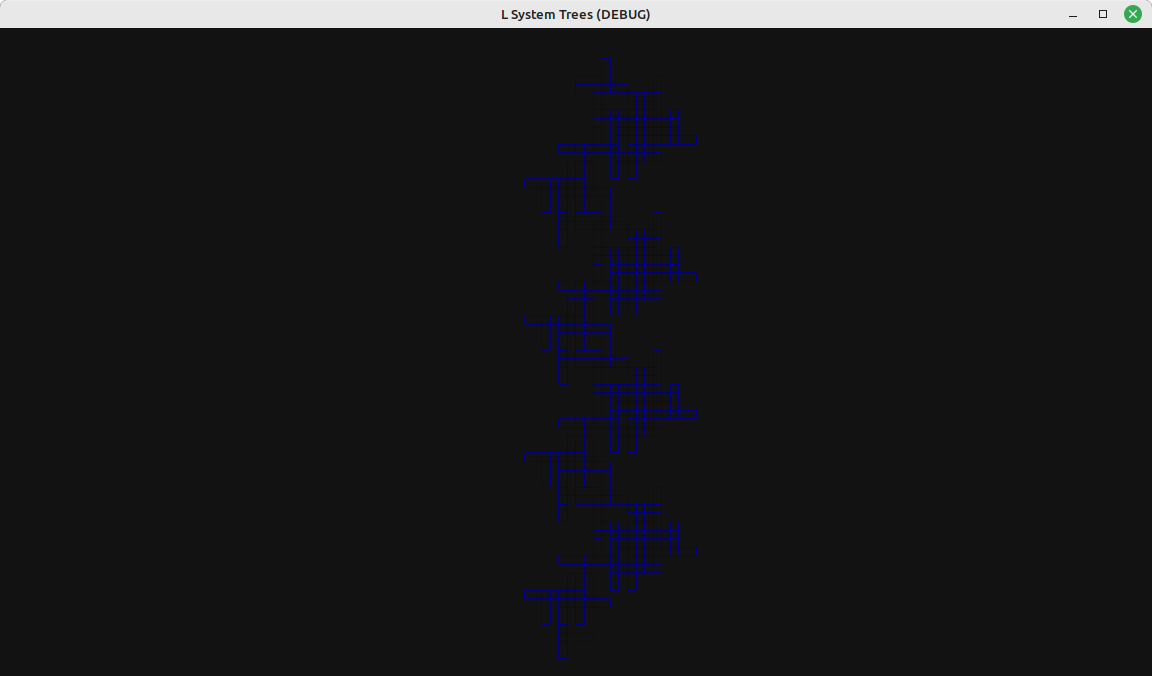
\includegraphics[width=0.75\textwidth]{Images/gd4lattice.png}
    \caption{A lattice generated with the example grammar on a Godot project for drawing from L-Systems. Source: Initial project written by YouTuber Codat\cite{codatGD3LSystemYT}\cite{codatGD3LSystemGH}, and converted to Godot 4 (with the addition of the lattice grammar) by me.\cite{codatGD4LSystemGH}}
    \label{fig:lattice2}
\end{figure}

\subsubsection{A More Complex D0L-System With More Than One Rule}

For handling more than one rule, we can instead use a new string buffer variable where, for each character in our string, we can attain a new string and append it to our string buffer. The resulting string is then returned and interpreted. This can be represented in Godot as demonstrated in Figure \ref{fig:lsys-snippet-2}, which uses two functions to perform string replacement. The first function \verb|get_new_replacement| performs the character replacement according to the L-System's grammar rules, while the second function \verb|replace_string| uses a string builder variable to allow for replacement of characters without directly affecting the original string and causing unwanted side effects.

\begin{figure}[H]
    \centering
    \begin{lstlisting}
func get_new_replacement(character: String) -> String:
	for rule in rules:
		if rule["from"] == character:
			return rule["to"]
	return character

func replace_string(string: String) -> String:
	var new_string = ""
	for character in string:
		new_string += get_new_replacement(character)
	return new_string
    \end{lstlisting}
    \caption{Two GDScript functions for replacing characters in an L-System grammar with more than one rule.}
    \label{fig:lsys-snippet-2}
\end{figure}

This can \textit{then} be used to handle more complex grammars that can handle more than one rule in which characters in strings are replaced by other strings of variable length, as before.

The grammar in the following example represents a D0L-System\cite{lsystemintro}, a \textbf{deterministic} L-System using a context-free grammar; the grammar in the first example was \textit{also} deterministic.

\newcommand{\A}{\mbox{a}}
\newcommand{\B}{\mbox{b}}

For this example, consider a new grammar $G$ with the alphabet $V$, where $\A$ and $\B$ are the only symbols. We start with the following axiom $\omega$, which is just $\A$. We now have a set of rules $P$ which is, this time, of size \textit{2}:

$$ \A \rightarrow \A\B $$
$$ \B \rightarrow \A $$

The first few steps of the resulting derivation can be modelled like so:

\begin{figure}[H]
    \centering
    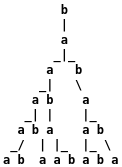
\includegraphics[scale=0.5]{Images/derivationtree.png}
    \caption{The first few steps of a derivation of our example grammar.\cite{lsystemintro}}
    \label{fig:derivationtree}
\end{figure}

\subsection{Perlin/Simplex Noise}

Traditionally, white noise images, and most other noise types, place noise pixels completely randomly, without each pixel considering the values of its neighbours\cite{gd3perlinnoise}, as you can see in Figure \ref{fig:whitenoisepic}.

However, there exists several types of \textbf{value} and \textbf{gradient} noise that \textit{do} take surrounding pixel values into consideration, and will therefore serve more use in building levels in our games.

Value noise simply takes a lattice of points with random values and then interpolates those points based on their surrounding values. This \textit{can} be used as a procedural texture. However, due to the simple nature of the algorithm, it's possible that the difference between several values in a region is minimal, while in other regions the values may differ immensely, resulting in a noise image that is not very smooth.

Gradient noise, on the other hand, takes point lattices and instead calculates the interpolation between tangents.\cite{perlinvalue} Since both tangents between a curve must be collinear\cite{perlinvalue}, the flat and bumpy curves produced by value noise's interpolation calculations are now much less likely to be returned, as seen in Figure \ref{fig:valueperlincomparison}.\cite{perlinvalue} This results in noise images of higher and more appealing visual quality as, to quote a response from Stack Exchange by Hernan J. González\cite{gradientvalue}, ``it cuts low frequencies and emphasizes frequencies around and above the grid spacing."

\begin{figure}[H]
    \centering
    
\includegraphics[width=\textwidth]{Images/whitenoisepic.png}
    \caption{A white noise picture generated with Robson's white noise image generator.\cite{whitenoisepicgen}\\Settings: 640 squares horizontally, 480 squares vertically, size of squares 1, colours greyscale, bias none.}
    \label{fig:whitenoisepic}
\end{figure}

\begin{figure}[H]
    \centering
    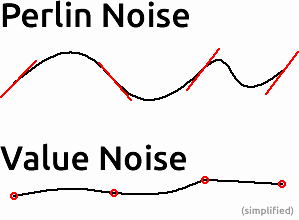
\includegraphics[width=\textwidth]{Images/valueperlincomparison.png}
    \caption{A comparison between the kinds of curves produced by Value noise interpolation and Perlin (and other Gradient) noise interpolation.\cite{perlinvalue}}
    \label{fig:valueperlincomparison}
\end{figure}

Two particularly well-known Gradient noise algorithms that are commonly used for procedurally generating levels are the already mentioned Perlin Noise and Simplex Noise, both designed by American Computer Science professor Kenneth H. Perlin, with the former being an improvement on the former. Perlin filed a patent on his work in 2002 that was granted in 2005\cite{perlinpatent}, which prompted the creation of the OpenSimplex noise algorithm\cite{enwiki:1102898483} for free use; the patent has since expired in 2022, allowing free use to both Perlin and the original Simplex noise.\cite{perlinpatent}

\subsection{Poisson Disk Sampling}

Poisson disk distributions are an easy way to randomly scatter objects across a field. It's commonly used for tree placement and placement of other random objects. Points are placed over a plane, with a single point placed randomly and subsequent points calculated such that a single point has no other point lying within a given radius of said point. Different implementations of Poisson disk distributions or samples can accommodate multiple radii for points in a plane, and some implementations produce \textit{maximal} samples- that is, a set of samples that fully cover the given plane, while still adhering to the principle that no single point has other points lying within its radius (the implementation I made for this project does \textbf{not} guarantee maximality, however).\\The following are some examples of Poisson disk distribution in action:

\begin{figure}[H]
    \centering
    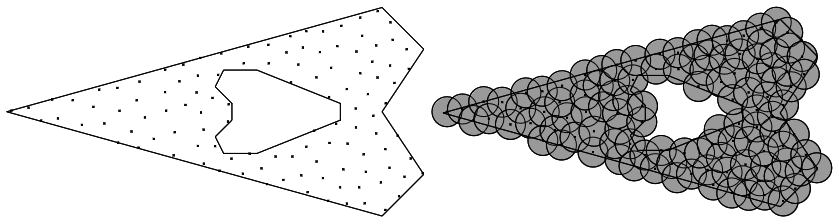
\includegraphics[width=\textwidth]{Images/maximalpoissonsample.png}
    \caption{A diagram of a maximal Poisson disk distribution done on a concave plane, with the right side denoting maximality through the grey disks overlapping but not any points overlapping.\cite{10.1145/1964921.1964944}}
    \label{fig:maximalpoisson}
\end{figure}

\begin{figure}[H]
    \centering
    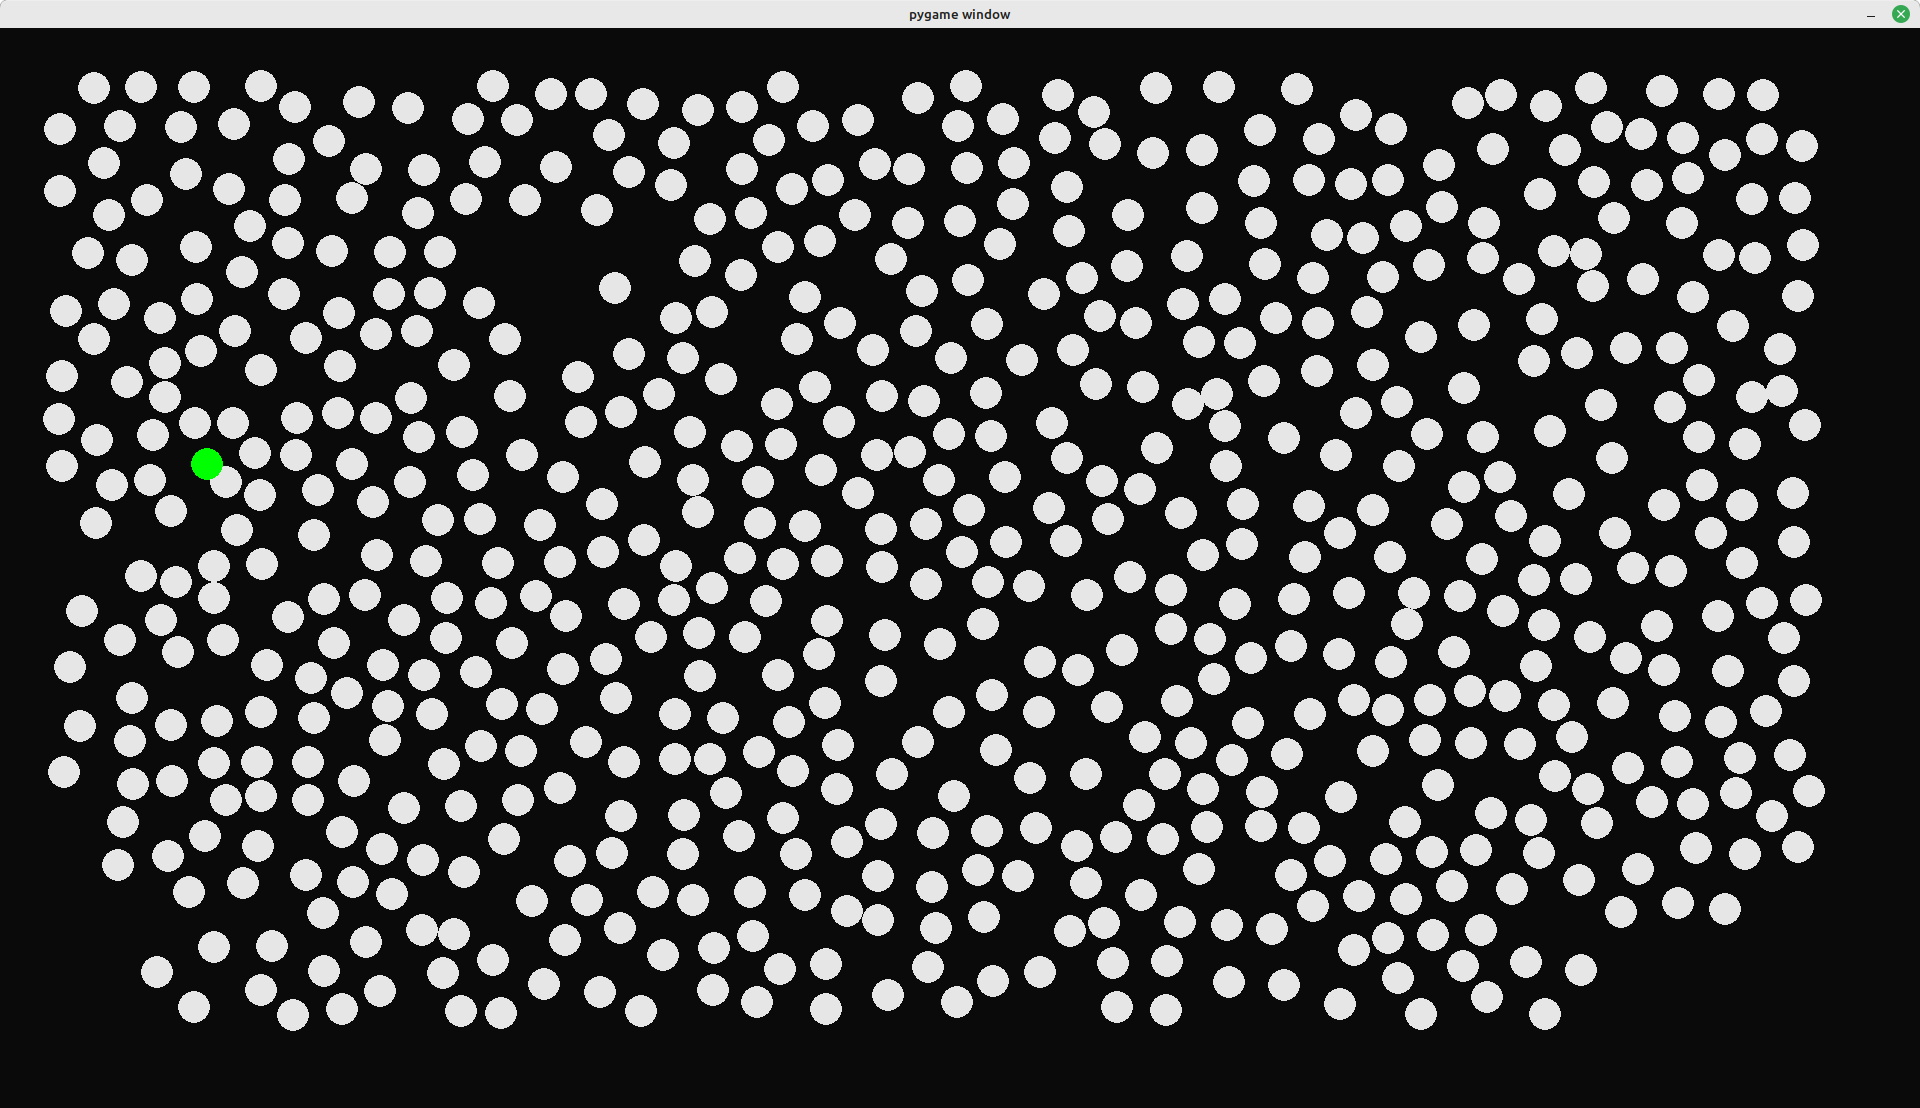
\includegraphics[width=\textwidth]{Images/pygamepoissonsample.png}
    \caption{An implementation of Poisson disk sampling made in Pygame.\cite{pygamepoissondisksampling} The screenshot was taken \textit{after} all of the samples were taken.}
    \label{fig:pygamepoisson}
\end{figure}

\subsection{Voronoï Cells}

Named after the Ukranian mathematician Georgy Voronoy, Voronoi cells work by taking a map of points, and randomly selecting a group of points. Within that selected group, cells are formed by calculating, in each point of the grid, the closest of the selected points to it. That is, each cell represents the group of points that are the closest to that random point (including that point in the group as well). The final arrangement of cells represents a Voronoi Diagram or Voronoi Tesselation.

Distances between points can be calculated with either the Euclidean distance:

$$ d_{E}(p, q) = \sqrt{(q_x - p_x)^2 + (q_y - p_y)^2} $$

or the Manhattan distance:

$$ d_{M}(p, q) = |q_x - p_x| + |q_y - p_y| $$

With the Euclidean distance producing a more ``triangulated" tesselation than the Manhattan distance, the geometry of which is more "blocky" and resembles taxicabs (hence its alternate name "Taxicab Geometry").

\section{Implementations}

Here I will describe, at surface level, the methods I went about implementing the above algorithms and what references I used.

\subsection{Lindenmayer System}

The implementation of an L-System was very simple. I took inspiration from a YouTube video on implementing an L-System for drawing line graphics in Godot by Codat.\cite{codatGD3LSystemYT} In the code from the Godot 3 project he made in that video\cite{codatGD3LSystemGH}\cite{codatGD3LSystemYT}, he created a custom ``Rule" class in GDScript, with which he defined new rules. I forked his project, converted it to Godot 4 and used it to create the lattice graphics in Figure \ref{fig:lattice2}. I did this mainly as a reference for my implementation of L-Systems in the game itself.

With the implementation in my \emph{game}, I adapted the \verb|get_new_character| method in that L-System to work with the dictionary I originally implemented my L-System in. The new \verb|get_new_replacement| method in my implementation allows for there to be more than one grammar rule while the L-System still performs as it should. My original L-System iterated through the original string \textit{directly}, which produced unintended consequences in grammars with multiple rules, as seen here when trying to implement the D0L-System I mentioned earlier\cite{lsystemintro}:

$$ b \rightarrow a \rightarrow aa \rightarrow aaa \rightarrow aaaa \rightarrow aaaaa \ldots $$

By using an empty string buffer and inserting rule replacements there instead, my implementation is now able to perform substitutions accordingly; the correct computation of the D0L-System is denoted in Figure \ref{fig:derivationtree} and repeated below:

$$ b \rightarrow a \rightarrow ab \rightarrow aba \rightarrow abaab \rightarrow abaababa \ldots $$

With the L-System string parsing algorithm in place, the next step was to paint the cells of each tile. With this, I iterated through every cell of the tilemap using a nested for-loop. With the parsed string, I then accessed the character of the string at an incremented index using an iterator variable I defined before the for-loops. The string consists of three different characters repeated multiple times, ``O", ``W" and ``B". For each string index, if the character is ``W", paint a tree, if it is ``B", paint a building, and if it is an ``O", leave the cell blank and paint nothing. The player and ring then get placed afterwards.

Even for a large-sized tile map with 2880 cells, a constant L-System $G$, with the symbols O, W and B and the following grammar

$$ \mbox{O} \rightarrow \mbox{O}\mbox{W}\mbox{O} $$
$$ \mbox{W} \rightarrow \mbox{W}\mbox{B} $$
$$ \mbox{B} \rightarrow \mbox{B}\mbox{W}\mbox{O} $$

can parse the axiom OWB, paint tile map tiles with the resulting string \textbf{and} place the player and ring in just a minimum of 19 milliseconds and a maximum of 22 milliseconds.

\subsection{Perlin/Simplex Noise}

The Simplex Noise implementation works with Godot's built-in Noise library. Within a Sprite2D node's Texture attribute, I set a new ``NoiseTexture2D" field inside of it. In its ``Noise" attribute I created a new ``FastNoiseLite" scene, which generates a noise texture for us to use. The seed can be set in the sprite's script file.

As with my other implementations, there are two separate arrays, one for trees and another for buildings. For each cell in the TileMap, I then took the noise pixel from the generated texture at that exact point (scaling with the cell size accordingly), using the \verb|get_noise_2d| method built-in with Godot, and then, depending on the value retrieved, decided, firstly, whether or not to place a plant/tree tile there and, secondly, whether or not to place a building tile there. As a result, not every cell in the TileMap has tiles on it. On any one of those empty cells, the Player tile will then get placed.

\subsection{Poisson Disk Sampling}

\subsection{Voronoï Cells}